\begin{lstlisting}[language=C++,caption={WiFi connect}, label=lst:wificonnect]
	bool wifiConnect(String ssid, String password)
	{
		//Verbindung initialisieren
		WiFi.begin(ssid, password);
		
		//Debug-Ausgabe
		Serial.print("\nConnecting to: ");
		Serial.print(ssid);
		
		//Auf erfolgreiche Verbindung warten
		while (WiFi.status() != WL_CONNECTED) { // Wait for the Wi-Fi to connect
			Serial.print(".");
			delay(1000);
		}
		
		//Debug-Ausgabe
		Serial.print("\nConnection established. IP: ");
		Serial.println(WiFi.localIP());
		Serial.println("===================================");
		
		return true;
	}
\end{lstlisting}

\begin{lstlisting}[language=C++,caption={MQTT Connect}, label=lst:mqttconnect]
	bool brokerConnect(const char *address, int port)
	{
		//Serveradresse und -port setzen
		client.setServer(address, port);
		
		//ClientID erzeugen
		String clientId = "HurensohnClient-";
		clientId += String(random(0xffff), HEX);
		
		Serial.print("Attempting MQTT connection");
		
		//Konsequent versuchen, eine Verbindung herzustellen
		while (!client.connected()) 
		{
			//Verbindung hergestellt, Schleife verlassen
			if(client.connect(clientId.c_str()))
			{
				std::cout << "\nBroker "<< brokerAddress <<" connected\n" << std::endl;
				return true;
			}
			//Verbinden fehlgeschlagen, nach 1s erneut versuchen
			else
			{
				Serial.print(".");
				//Serial.println(client.state());
				delay(1000);
			}
		}
		return true;
	}
\end{lstlisting}

\begin{lstlisting}[language=C++,caption={Write Json}, label=lst:writejson]
	serializedData["device\_id"]   = ESP\_ID;
	serializedData["timestamp"]   = currData->timestamp;
	serializedData["temperature"] = currData->temperature;
	serializedData["humidity"]    = currData->humidity;
	serializedData["altitude"]    = currData->altitude;
	serializedData["airPressure"] = currData->airPressure;
\end{lstlisting}

\begin{figure}[h]
	\centering
	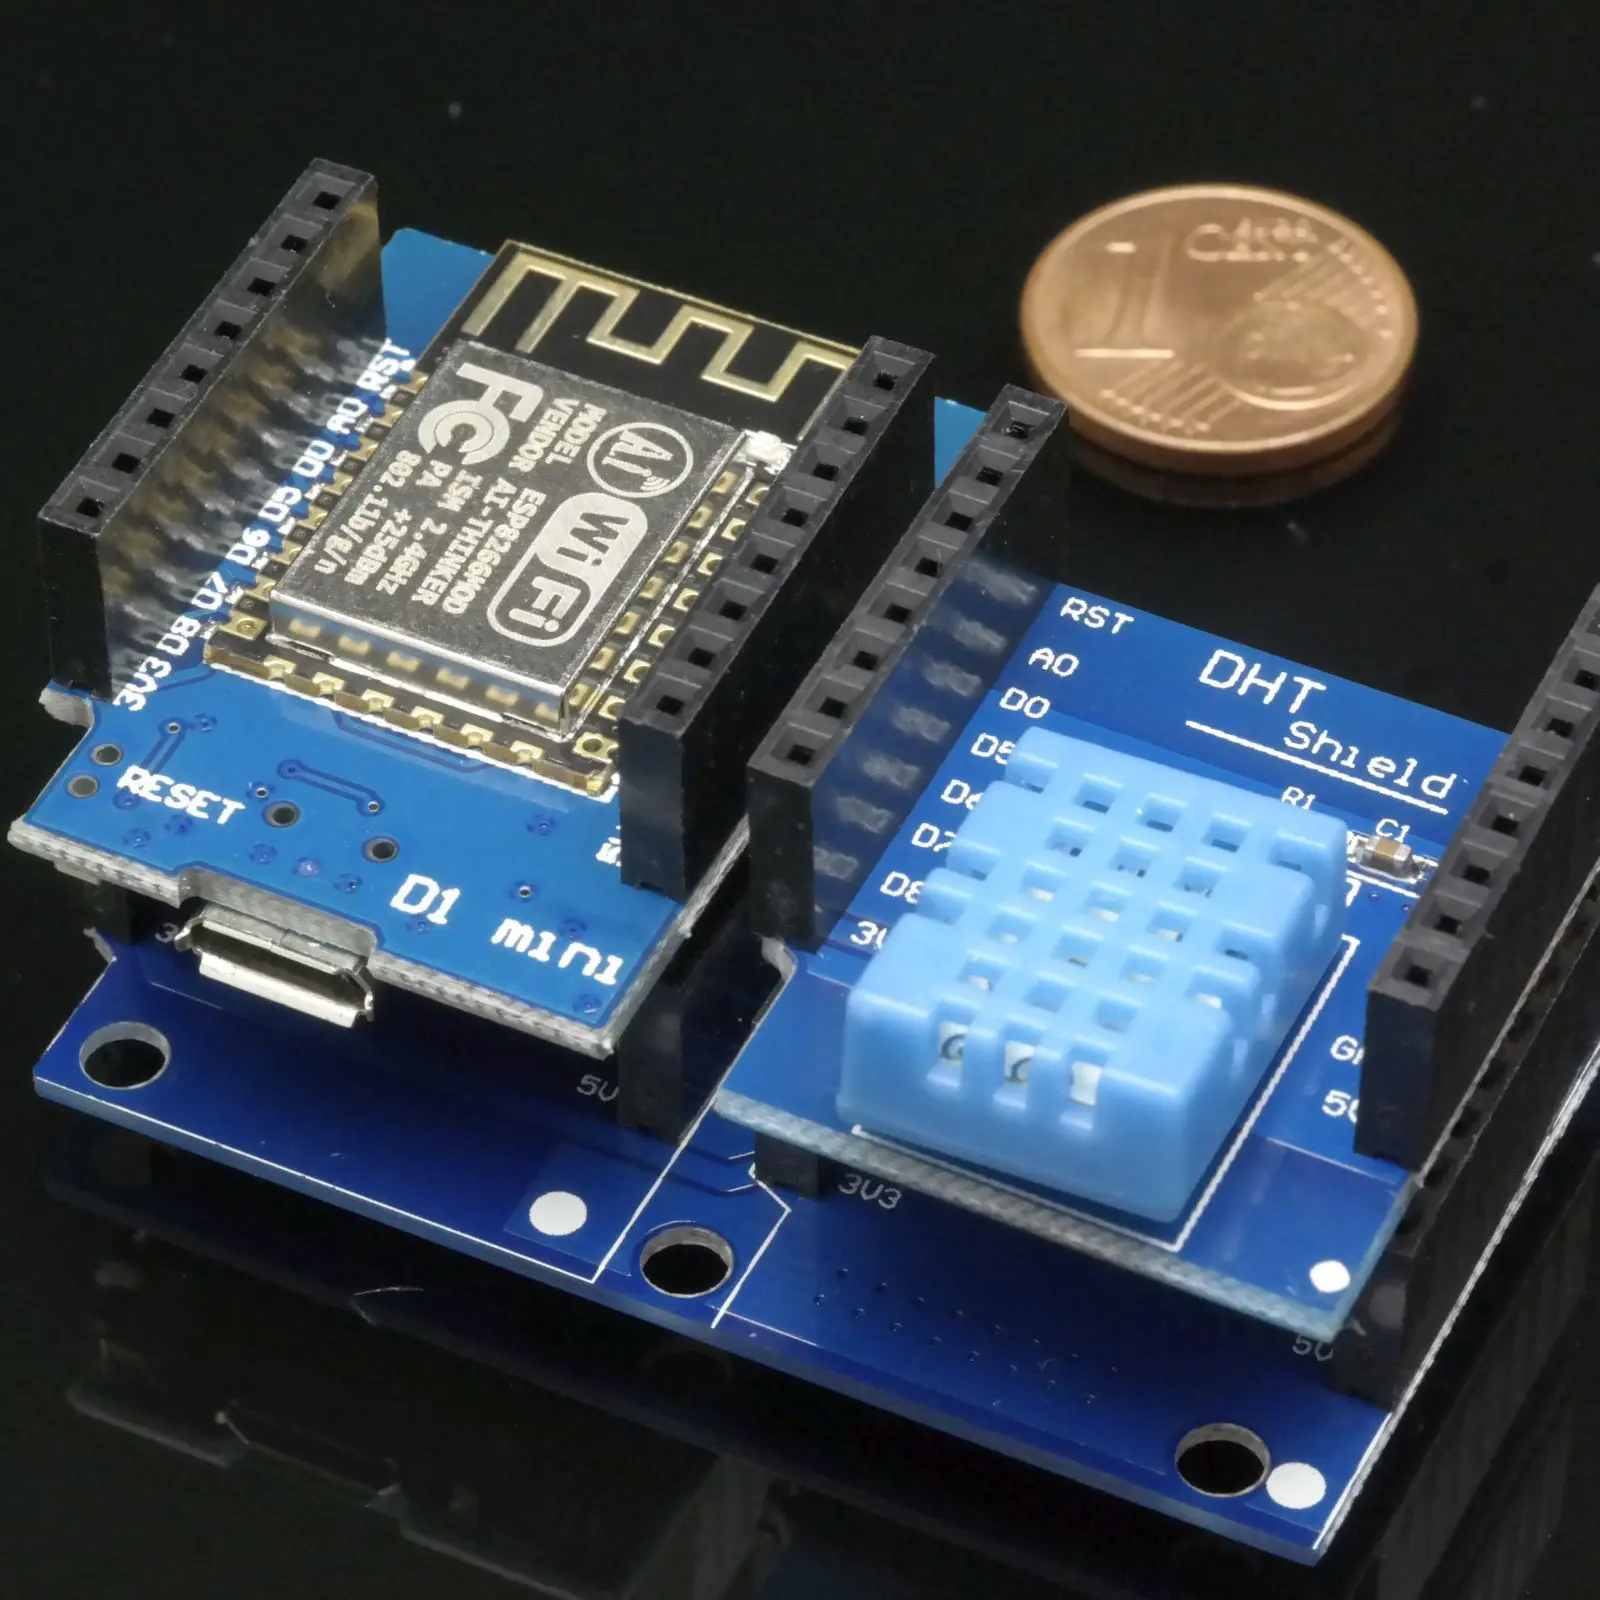
\includegraphics[width=7cm]{images/esp_dht.png}
	\caption[dht\_an\_esp]{DHT an ESP8266 angesteckt}
	\label{fig:dht_an_esp}
\end{figure}